% !Mode:: "TeX:UTF-8"
% !TEX program  = xelatex
\documentclass[a4paper]{article}
\usepackage{amsmath}
\usepackage{amssymb}
\usepackage{ctex}
\usepackage{graphicx}
\usepackage[european]{circuitikz}
\usepackage{multirow}
\usepackage{geometry}
\usepackage{hyperref}
\geometry{a4paper, top=2.54cm, bottom=2.54cm, left=2.54cm, right=2.54cm}
\title{编程作业一报告}
\author{王凯灵 521030910356}
\date{2023年2月15日}
\begin{document}
	\maketitle
	本次作业要求使用点扩散函数将一张图片模糊化、添加噪声以后尝试使用逆滤波和Wiener滤波去噪、去模糊。
	
	\section{步骤一}
	在matlab中，使用imread函数读取图片"baboon.bmp"，使用fspecial函数定义PSF矩阵，使用conv2函数进行二维卷积，将转化为uint8的卷积结果保存为图片，原始图像和模糊化结果如original image(图\ref{oi})和blurred image(图\ref{bi})。使用imfilter可以得到类似的效果，但conv2更加直观。保存结果的时候，我保留了大部分的图片，但我去处了一部分，因为只有这样，输出的尺寸才能和原图保持一致，考虑到现实情况，这样更加合理。与要求中给出的图相比，发现要求中的结果图更亮。为了消除视觉误差，从pdf中进行了像素级别的图像分离并比较能量，发现要求中模糊后的图像能量大于原图，推测给出的图有误。后已在课程群中解决。
	
	\section{步骤二}
	使用awgn函数，所得结果分别如blurred and noised in 30dB(图\ref{n30})、blurred and noised in 20dB(图\ref{n20})和blurred and noised in 10dB(图\ref{n10})所示。观察发现所得图像颗粒感严重，而要求的图片中，没有这么严重的颗粒感。推测pdf制作时图像可能发生了损失。
	
	作业要求中提到，有多种方法可以添加噪声，并给出了awgn和imnoise作为参考。阅读awgn的代码发现，按照我的使用方法，awgn先计算输入的能量，再使用randn生成高斯噪声，按给定的SNR将噪声加入输入信号并输出。imnoise使用了库函数images.internal.algimnoise，同样使用randn生成噪声。理论上二者效果相同。
	
	\section{步骤三}
	使用deconvlucy函数进行直接逆滤波。代码中，另外给出了使用fft的版本。效果如图\ref{rd30}，\ref{rd20}，\ref{rd10}所示。使用Wiener滤波，结果如图\ref{rw30}，\ref{rw20}，\ref{rw10}所示。另外，给出了lucy变换(报告中未显示)，观察所得结果，认为从视觉角度上来说，维纳滤波的结果更平滑，在20dB的图像上，维纳滤波的优势体现的十分明显。
	
	\newgeometry{top=1cm, bottom=0cm, left=2cm, right=2cm}
	\section{附录：图片}
	\begin{figure}[h!]
		\begin{minipage}[t]{0.5\linewidth}
			\centering
			
\includegraphics[width=0.576\textwidth]{../code/baboon}
			\caption{original image}
			\label{oi}
		\end{minipage}
		\begin{minipage}[t]{0.5\linewidth}
			\centering
			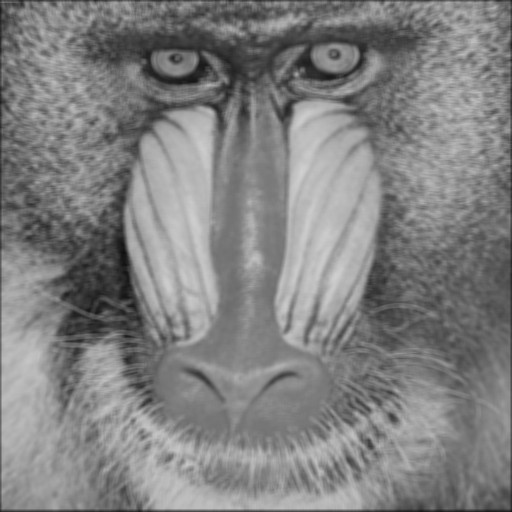
\includegraphics[width=0.576\textwidth]{figures/baboon_blur}
			\caption{blurred image}
			\label{bi}
		\end{minipage}
	\end{figure}
	\begin{figure}[h!]
		\begin{minipage}[t]{0.32\linewidth}
			\centering
			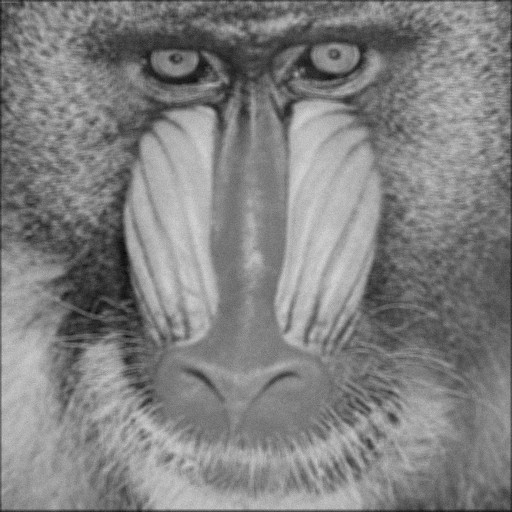
\includegraphics[width=0.9\textwidth]{figures/baboon_30}
			\caption{blurred and noised in 30dB}
			\label{n30}
		\end{minipage}
		\begin{minipage}[t]{0.32\linewidth}
			\centering
			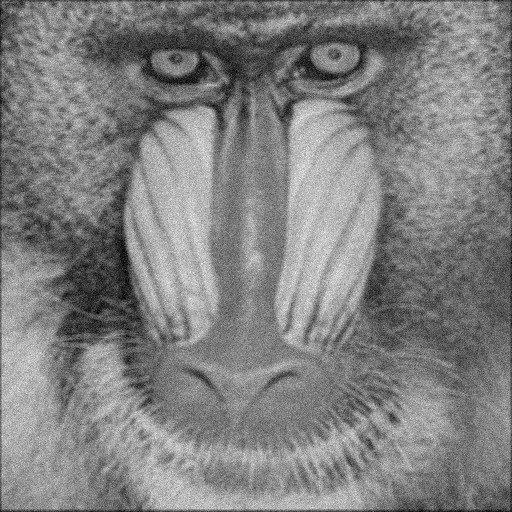
\includegraphics[width=0.9\textwidth]{figures/baboon_20}
			\caption{blurred and noised in 20dB}
			\label{n20}	
		\end{minipage}
		\begin{minipage}[t]{0.32\linewidth}
			\centering
			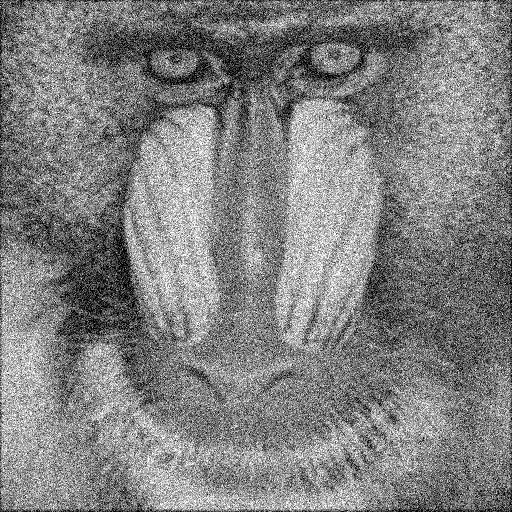
\includegraphics[width=0.9\textwidth]{figures/baboon_10}
			\caption{blurred and noised in 10dB}
			\label{n10}
		\end{minipage}
	\end{figure}
	\begin{figure}[h!]
		\begin{minipage}[t]{0.32\linewidth}
			\centering
			
\includegraphics[width=0.9\textwidth]{figures/rd_baboon_30}
			\caption{directly restore 30dB}
			\label{rd30}
		\end{minipage}
		\begin{minipage}[t]{0.32\linewidth}
			\centering
			
\includegraphics[width=0.9\textwidth]{figures/rd_baboon_20}
			\caption{directly restore 20dB}
			\label{rd20}	
		\end{minipage}
		\begin{minipage}[t]{0.32\linewidth}
			\centering
			
\includegraphics[width=0.9\textwidth]{figures/rd_baboon_10}
			\caption{directly restore 10dB}
			\label{rd10}
		\end{minipage}
	\end{figure}
	\begin{figure}[h!]
		\begin{minipage}[t]{0.32\linewidth}
			\centering
			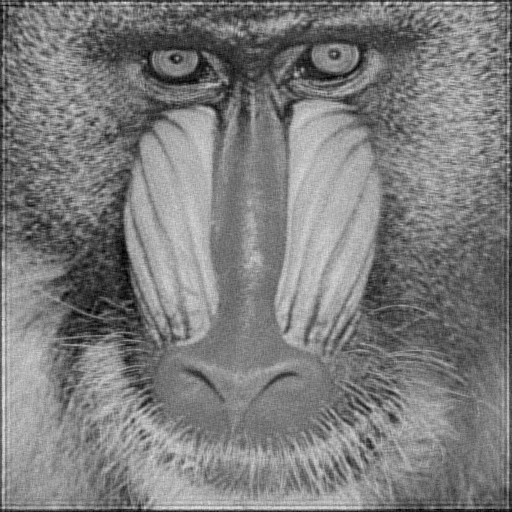
\includegraphics[width=0.9\textwidth]{figures/rw_baboon_30}
			\caption{Wiener restore 30dB}
			\label{rw30}
		\end{minipage}
		\begin{minipage}[t]{0.32\linewidth}
			\centering
			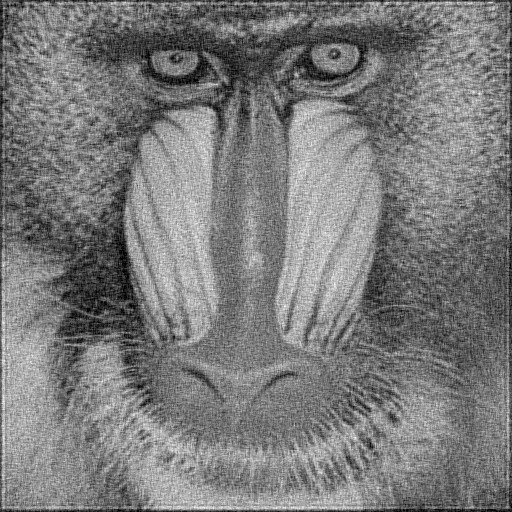
\includegraphics[width=0.9\textwidth]{figures/rw_baboon_20}
			\caption{Wiener restore 20dB}
			\label{rw20}	
		\end{minipage}
		\begin{minipage}[t]{0.32\linewidth}
			\centering
			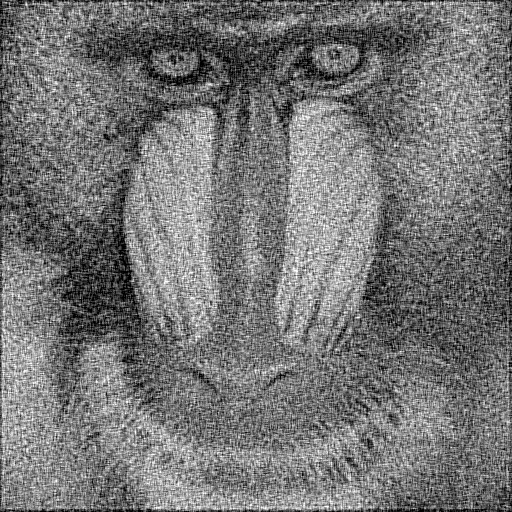
\includegraphics[width=0.9\textwidth]{figures/rw_baboon_10}
			\caption{Wiener restore 10dB}
			\label{rw10}
		\end{minipage}
	\end{figure}
	\newgeometry{top=2.54cm, bottom=2.54cm, left=2.54cm, right=2.54cm}
	\section{免责声明}
		本次作业过程中，包含解题、代码、报告等，无Chat-GPT或同类工具协助。
\end{document}